\chapter{Managing LVM Logical Volumes}

\section{Why use LVM}
LVM provides a flexible approach to storage:

\vspace{-10pt}
\begin{itemize}
	\item Volumes can consist of more than one disk.
	\item Volumes can be made smaller or larger easily.
	\item It is easy to replace failing disks.
	\item Provides advanced options like working with snapshots - a method by which backups can be made of files while they're open!
	\item It is easy to add many new volumes. While with partitions, there is a limit of 15 partitions, there can be as many as 256 logical volumes. 
\end{itemize}

\section{Understanding LVM Setup}
When working with LVM, we always start with physical storage media such as a hard disk (\textit{sda}). Typically, a partition on the hard disk is marked as the physical volume. Now, this physical volume is added to the \textbf{volume group} which is essentially an abstraction of all the storage available. Thus, all logical volumes are created from this volume group, and from their perspective, the physical volume that's acting as it's storage media isn't important. 

Once the logical volume is made from the storage in the volume group, we get a device called \verb|/dev/vgroup/logvol|. This is the device for the logical volume on which we create the file system. As long as there is space on the volume group, we can add new logical volumes on it. If there isn't we can also add a physical volume to the volume group, to increase its capacity. 

\begin{figure}[H]
	\centering
	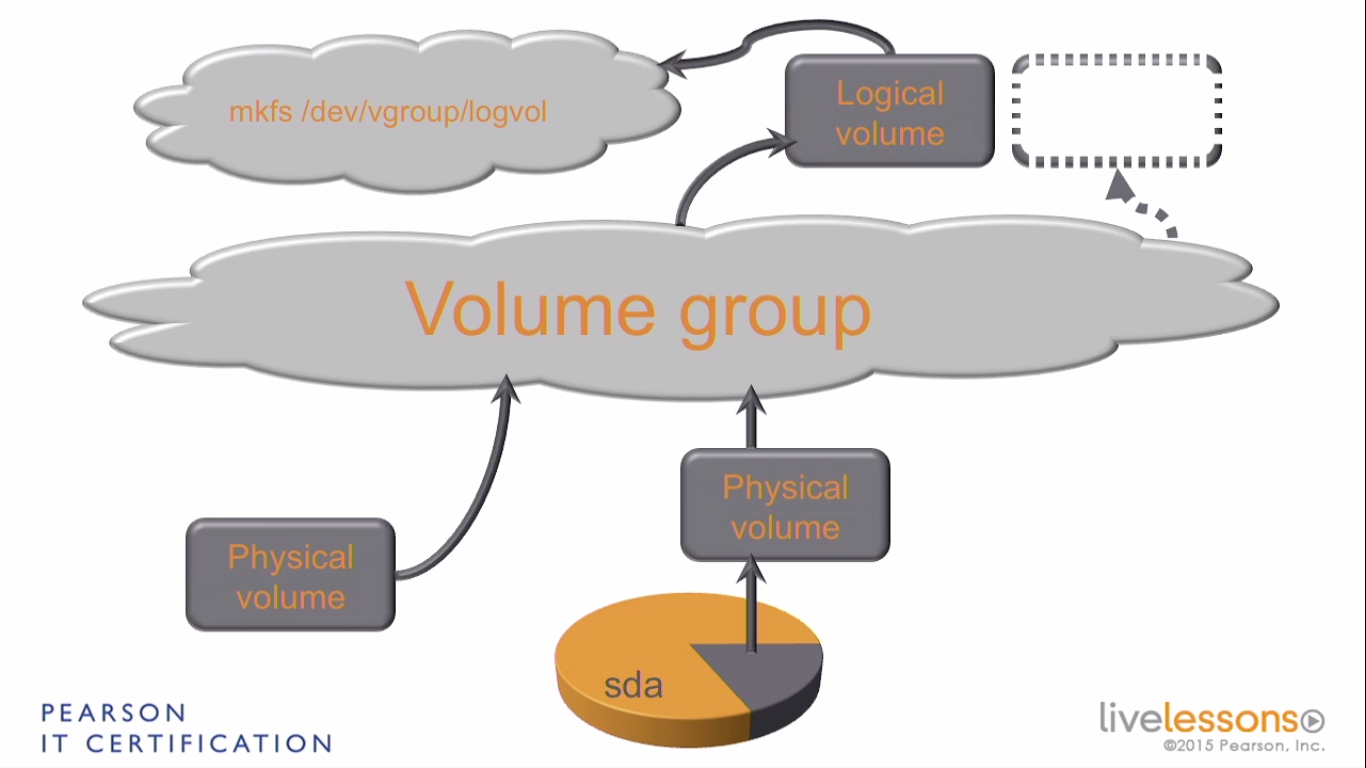
\includegraphics[width=0.9\linewidth]{Mod2/chapters/2.16.a}
	\caption{LVM Setup}
	\label{fig:2 LVM Setup}
\end{figure}

\section{Creating an LVM Logical Volume}

To create a new LVM partition, first we need to make a partition like any other partition. 

\vspace{-15pt}
\begin{minted}{console}
# fdisk /dev/sdb
Welcome to fdisk (util-linux 2.23.2).

Changes will remain in memory only, until you decide to write them.
Be careful before using the write command.


Command (m for help): p

Disk /dev/sdb: 10.7 GB, 10737418240 bytes, 20971520 sectors
Units = sectors of 1 * 512 = 512 bytes
Sector size (logical/physical): 512 bytes / 512 bytes
I/O size (minimum/optimal): 512 bytes / 512 bytes
Disk label type: dos
Disk identifier: 0xf11ab429

Device Boot      Start         End      Blocks   Id  System
/dev/sdb1            2048     4196351     2097152    5  Extended
/dev/sdb5            4096     2101247     1048576   83  Linux
/dev/sdb6         2103296     4196351     1046528   83  Linux

Command (m for help): n
Partition type:
p   primary (0 primary, 1 extended, 3 free)
l   logical (numbered from 5)
Select (default p): p
Partition number (2-4, default 2): 
First sector (4196352-20971519, default 4196352): 
Using default value 4196352
Last sector, +sectors or +size{K,M,G} (4196352-20971519, default 20971519): +100M 
Partition 2 of type Linux and of size 100 MiB is set

Command (m for help): p

Disk /dev/sdb: 10.7 GB, 10737418240 bytes, 20971520 sectors
Units = sectors of 1 * 512 = 512 bytes
Sector size (logical/physical): 512 bytes / 512 bytes
I/O size (minimum/optimal): 512 bytes / 512 bytes
Disk label type: dos
Disk identifier: 0xf11ab429

Device Boot      Start         End      Blocks   Id  System
/dev/sdb1            2048     4196351     2097152    5  Extended
/dev/sdb2         4196352     4401151      102400   83  Linux
/dev/sdb5            4096     2101247     1048576   83  Linux
/dev/sdb6         2103296     4196351     1046528   83  Linux
# fdisk /dev/sdb
Welcome to fdisk (util-linux 2.23.2).

Changes will remain in memory only, until you decide to write them.
Be careful before using the write command.


Command (m for help): p

Disk /dev/sdb: 10.7 GB, 10737418240 bytes, 20971520 sectors
Units = sectors of 1 * 512 = 512 bytes
Sector size (logical/physical): 512 bytes / 512 bytes
I/O size (minimum/optimal): 512 bytes / 512 bytes
Disk label type: dos
Disk identifier: 0xf11ab429

Device Boot      Start         End      Blocks   Id  System
/dev/sdb1            2048     4196351     2097152    5  Extended
/dev/sdb5            4096     2101247     1048576   83  Linux
/dev/sdb6         2103296     4196351     1046528   83  Linux

Command (m for help): n
Partition type:
p   primary (0 primary, 1 extended, 3 free)
l   logical (numbered from 5)
Select (default p): p
Partition number (2-4, default 2): 
First sector (4196352-20971519, default 4196352): 
Using default value 4196352
Last sector, +sectors or +size{K,M,G} (4196352-20971519, default 20971519): +100M 
Partition 2 of type Linux and of size 100 MiB is set

Command (m for help): p

Disk /dev/sdb: 10.7 GB, 10737418240 bytes, 20971520 sectors
Units = sectors of 1 * 512 = 512 bytes
Sector size (logical/physical): 512 bytes / 512 bytes
I/O size (minimum/optimal): 512 bytes / 512 bytes
Disk label type: dos
Disk identifier: 0xf11ab429

Device Boot      Start         End      Blocks   Id  System
/dev/sdb1            2048     4196351     2097152    5  Extended
/dev/sdb2         4196352     4401151      102400   83  Linux
/dev/sdb5            4096     2101247     1048576   83  Linux
/dev/sdb6         2103296     4196351     1046528   83  Linux
\end{minted}
\vspace{-10pt}

\noindent
Now that we have specified the details of our new partition, we need to change one more before we can use the LVM partitions. We enter the command \verb|t| to change the partition type, and then show the overview of all the acceptable partition types using \verb|l|. From the command below, we can see that there is a partition type called \textbf{Linux LVM} which suits our requirements. 

\vspace{-15pt}
\begin{minted}{console}
Command (m for help): t
Partition number (1,2,5,6, default 6): 2
Hex code (type L to list all codes): L

0  Empty           24  NEC DOS         81  Minix / old Lin bf  Solaris        
1  FAT12           27  Hidden NTFS Win 82  Linux swap / So c1  DRDOS/sec (FAT-
2  XENIX root      39  Plan 9          83  Linux           c4  DRDOS/sec (FAT-
3  XENIX usr       3c  PartitionMagic  84  OS/2 hidden C:  c6  DRDOS/sec (FAT-
4  FAT16 <32M      40  Venix 80286     85  Linux extended  c7  Syrinx         
5  Extended        41  PPC PReP Boot   86  NTFS volume set da  Non-FS data    
6  FAT16           42  SFS             87  NTFS volume set db  CP/M / CTOS / .
7  HPFS/NTFS/exFAT 4d  QNX4.x          88  Linux plaintext de  Dell Utility   
8  AIX             4e  QNX4.x 2nd part 8e  Linux LVM       df  BootIt         
9  AIX bootable    4f  QNX4.x 3rd part 93  Amoeba          e1  DOS access     
a  OS/2 Boot Manag 50  OnTrack DM      94  Amoeba BBT      e3  DOS R/O        
b  W95 FAT32       51  OnTrack DM6 Aux 9f  BSD/OS          e4  SpeedStor      
c  W95 FAT32 (LBA) 52  CP/M            a0  IBM Thinkpad hi eb  BeOS fs        
e  W95 FAT16 (LBA) 53  OnTrack DM6 Aux a5  FreeBSD         ee  GPT            
f  W95 Ext'd (LBA) 54  OnTrackDM6      a6  OpenBSD         ef  EFI (FAT-12/16/
10  OPUS            55  EZ-Drive        a7  NeXTSTEP        f0  Linux/PA-RISC b
11  Hidden FAT12    56  Golden Bow      a8  Darwin UFS      f1  SpeedStor      
12  Compaq diagnost 5c  Priam Edisk     a9  NetBSD          f4  SpeedStor      
14  Hidden FAT16 <3 61  SpeedStor       ab  Darwin boot     f2  DOS secondary  
16  Hidden FAT16    63  GNU HURD or Sys af  HFS / HFS+      fb  VMware VMFS    
17  Hidden HPFS/NTF 64  Novell Netware  b7  BSDI fs         fc  VMware VMKCORE 
18  AST SmartSleep  65  Novell Netware  b8  BSDI swap       fd  Linux raid auto
1b  Hidden W95 FAT3 70  DiskSecure Mult bb  Boot Wizard hid fe  LANstep        
1c  Hidden W95 FAT3 75  PC/IX           be  Solaris boot    ff  BBT            
1e  Hidden W95 FAT1 80  Old Minix      
Hex code (type L to list all codes): 8e
Changed type of partition 'Linux' to 'Linux LVM'

Command (m for help): p

Disk /dev/sdb: 10.7 GB, 10737418240 bytes, 20971520 sectors
Units = sectors of 1 * 512 = 512 bytes
Sector size (logical/physical): 512 bytes / 512 bytes
I/O size (minimum/optimal): 512 bytes / 512 bytes
Disk label type: dos
Disk identifier: 0xf11ab429

Device Boot      Start         End      Blocks   Id  System
/dev/sdb1            2048     4196351     2097152    5  Extended
/dev/sdb2         4196352     4401151      102400   8e  Linux LVM
/dev/sdb5            4096     2101247     1048576   83  Linux
/dev/sdb6         2103296     4196351     1046528   83  Linux

Command (m for help): w
The partition table has been altered!

Calling ioctl() to re-read partition table.

WARNING: Re-reading the partition table failed with error 16: Device or resource busy.
The kernel still uses the old table. The new table will be used at
the next reboot or after you run partprobe(8) or kpartx(8)
Syncing disks.
# partprobe
\end{minted}
\vspace{-10pt}

\noindent
We enter the value \verb|8e| since it's the code for the Linux LVM partition that we need. Finally, we use \verb|p| to print the partition table and verify our partition, \verb|w| to save the changes and \verb|partprobe| to push the changes to the kernel. 

\subsection{Creating a Physical Volume}
A physical volume is just a partition with the LVM metadata added to it. The volume groups built from the PVs are not possible to build without this metadata stored in the partitions. The physical volumes are created using \verb|pvcreate|. We can show all physical volumes using \verb|pvs|. 

\vspace{-15pt}
\begin{minted}{console}
# pvcreate /dev/sdb2
Physical volume "/dev/sdb2" successfully created.
# pvs
PV         VG     Fmt  Attr PSize   PFree  
/dev/sda3  centos lvm2 a--  <14.91g   4.00m
/dev/sdb2         lvm2 ---  100.00m 100.00m
\end{minted}
\vspace{-10pt}

\noindent
The \verb|pvs| command tells us that we have a physical volume called \verb|/dev/sdb2| which isn't in a volume group yet, has a LVM2 formatting, has a partition size of 100MB and has the same amount of free space. 

\subsection{Creating a Volume Group}

Next, we create a new volume group using the \verb|vgcreate| command. Again, we can check the volume groups on our system using the \verb|vgs| command. 

\vspace{-15pt}
\begin{minted}{console}
# vgcreate vgPrime /dev/sdb2
Volume group "vgPrime" successfully created
# vgs
VG      #PV #LV #SN Attr   VSize   VFree 
centos    1   4   0 wz--n- <14.91g  4.00m
vgPrime   1   0   0 wz--n-  96.00m 96.00m
\end{minted}
\vspace{-10pt}

\noindent
The volume group \textit{vgPrime} has 1 PV in it (\textit{/dev/sda2}), no logical volumes, And has a Volume size of 96MB, all of which is free!

\subsection{Creating a Logical Volume}
The creating of a Logical Volume on a VG requires specifying the size of the logical volume. This can be done in two ways: by counting the number of extents (building blocks of LVM) [\verb|-l|] or the actual size on disk (KB, MB, GB, TB, etc.)[\verb|-L|]. Finally, we also can provide the name of the LV using the \verb|-n| option. 

\vspace{-15pt}
\begin{minted}{console}
# lvcreate -n lvPrime -L 96M vgPrime
Logical volume "lvPrime" created.
# lvs
LV      VG      Attr       LSize  Pool Origin Data%  Meta%  Move Log Cpy%Sync Convert
home    centos  -wi-ao----  7.45g                                                    
root    centos  -wi-ao----  3.72g                                                    
swap    centos  -wi-ao----  1.86g                                                    
var     centos  -wi-ao----  1.86g                                                    
lvPrime vgPrime -wi-a----- 96.00m                
\end{minted}
\vspace{-10pt}

\subsection{Creating a File system on the LV}
Now, since the LV is ready, we can put a file system on it. We refer to the logical volume device by \verb|/dev/<volumeGroupName>/<logicalVolumeName>|.

\vspace{-15pt}
\begin{minted}{console}
# mkfs.ext2 /dev/vgPrime/lvPrime
mke2fs 1.42.9 (28-Dec-2013)
Filesystem label=
OS type: Linux
Block size=1024 (log=0)
Fragment size=1024 (log=0)
Stride=0 blocks, Stripe width=0 blocks
24576 inodes, 98304 blocks
4915 blocks (5.00%) reserved for the super user
First data block=1
Maximum filesystem blocks=67371008
12 block groups
8192 blocks per group, 8192 fragments per group
2048 inodes per group
Superblock backups stored on blocks: 
8193, 24577, 40961, 57345, 73729

Allocating group tables: done                            
Writing inode tables: done                            
Writing superblocks and filesystem accounting information: done 

# mount /dev/vgPrime/lvPrime /mnt
# mount | grep ^/dev/
/dev/mapper/centos-root on / type xfs (rw,relatime,seclabel,attr2,inode64,noquota)
/dev/sdb5 on /data type ext4 (rw,relatime,seclabel,data=ordered)
/dev/mapper/centos-var on /var type xfs (rw,relatime,seclabel,attr2,inode64,noquota)
/dev/mapper/centos-home on /home type xfs (rw,relatime,seclabel,attr2,inode64,noquota)
/dev/sda2 on /boot type xfs (rw,relatime,seclabel,attr2,inode64,noquota)
/dev/sr0 on /run/media/somu/CentOS 7 x86_64 type iso9660 (ro,nosuid,nodev,relatime,uid=1000,gid=1000,iocharset=utf8,mode=0400,dmode=0500,uhelper=udisks2)
/dev/mapper/vgPrime-lvPrime on /mnt type ext2 (rw,relatime,seclabel)
\end{minted}
\vspace{-10pt}

\noindent
Here, we can see that there is a strange behavior with the device that is mounted. While we issued the command to mount \verb|/dev/vgPrime/lvPrime|, the device that was actually mounted is shown as \verb|/dev/mapper/vgPrime-lvPrime|. This is because both those names are symlinks to the real name of the device (\textit{dm-5}):

\vspace{-15pt}
\begin{minted}{console}
# ls -l /dev/mapper/vgPrime-lvPrime /dev/vgPrime/lvPrime
lrwxrwxrwx. 1 root root 7 Dec 11 15:13 /dev/mapper/vgPrime-lvPrime -> ../dm-5
lrwxrwxrwx. 1 root root 7 Dec 11 15:13 /dev/vgPrime/lvPrime -> ../dm-5
\end{minted}
\vspace{-10pt}

\noindent
The device \verb|/dev/dm-5| is a Device Mapper device, which is the same as used in case of LUKS encrypted volumes. 

\section{Understanding Device Mapper and LVM Device Names}
The device mapper is an abstraction layer that the kernel works with to communicate with certain types of storage devices. Both LUKS encrypted partitions and LVM use the device mapper. Other devices such as software RAID and multipath also have to communicate via the device mapper. 

Contrastingly, the XFS, Ext4, etc file systems work with the help of the VFS (Virtual File System) layer (instead of the Device Mapper abstraction layer). The device mapper has the devices present as \verb|dm-*| (\textit{dm-0, dm-1, etc.}) but we shouldn't use them. The names are assigned during boot, and are subject to change at any time! This is why the device mapper provides a bunch of symlinks to the related devices in the \verb|/device/mapper| directory. They are: \verb|/dev/mapper/vg-lv| and \verb|/dev/vg/lv| which are both symlinks to the same device. 

\section{Understanding LVM resize operations}
The structure of LVMs are simple: the file system (FS) are installed on Logical Volumes (LV). These Logical Volumes get their disk space from Volume Groups (VG) which use several Physical Volumes (PV) that actually hold the data and provides the disk space. 

\subsection{Extending the File System}
To expand the disk capacity of the file system, we need more space in the Logical volume. This means that (possibly) more space has to be added to the Volume Group itself, and thus, more physical volumes may need to be added. 

So, first we need to create a new physical volume, and then assign it to the volume group. Then it is possible to grow the logical volume, and finally extend the file system. 

\subsection{Shrinking the File System}
At first we have to reduce the size of the file system, and then reduce the size of the logical volume. If we don't there will be a file system with a bigger size than the logical partition it's residing on. 

Thus, after reducing the file system size and then the logical volume size, we can then reduce the size of the volume group (if needed). 

\section{Growing an LVM Logical Volume}
We can grow the LVM volume if we're running out of disk space and want to make it bigger. We typically check the amount of free space using \verb|df -h| (\textit{disk free - human-readable}) command:

\vspace{-15pt}
\begin{minted}{console}
# df -h
Filesystem                   Size  Used Avail Use% Mounted on
/dev/mapper/centos-root      3.8G  3.6G  163M  96% /
devtmpfs                     2.9G     0  2.9G   0% /dev
tmpfs                        2.9G     0  2.9G   0% /dev/shm
tmpfs                        2.9G  9.1M  2.9G   1% /run
tmpfs                        2.9G     0  2.9G   0% /sys/fs/cgroup
/dev/sdb5                    976M  2.6M  907M   1% /data
/dev/mapper/centos-var       1.9G  365M  1.5G  20% /var
/dev/mapper/centos-home      7.5G   68M  7.4G   1% /home
/dev/sda2                    485M  266M  220M  55% /boot
tmpfs                        580M  4.0K  580M   1% /run/user/42
tmpfs                        580M   36K  580M   1% /run/user/1000
/dev/sr0                     8.1G  8.1G     0 100% /run/media/somu/CentOS 7 x86_64
/dev/mapper/vgPrime-lvPrime   93M  1.6M   87M   2% /mnt
\end{minted}
\vspace{-10pt}

\noindent
Now, since it's an LVM, the order in which we grow the different components matter. To make the filesystem bigger, first we check the LV size and then check to see if there's any free space in the VG:

\vspace{-15pt}
\begin{minted}{console}
# lvs
LV    VG               Attr       LSize   Pool Origin Data%  Meta%  Move Log Cpy%Sync Convert
root  centos_cliserver -wi-ao---- <17.00g                                                    
swap  centos_cliserver -wi-ao----   2.00g                                                    
lvCLI vgCLI            -wi-a----- 100.00m                                                    
# vgs
VG               #PV #LV #SN Attr   VSize   VFree  
centos_cliserver   1   2   0 wz--n- <19.00g      0 
vgCLI              2   1   0 wz--n- 192.00m  92.00m
\end{minted}
\vspace{-10pt}

\noindent
From the last line of the command, we can see that vgPrime has 0 VFree (i.e., free space in the VG). Thus, we need to work bottom up and make it bigger before we can make the LV and the FS bigger. So, we run \verb|fdisk| on \textit{/dev/sdb}.

\vspace{-15pt}
\begin{minted}{console}
# fdisk /dev/sdb
Welcome to fdisk (util-linux 2.23.2).

Changes will remain in memory only, until you decide to write them.
Be careful before using the write command.


Command (m for help): p

Disk /dev/sdb: 4294 MB, 4294967296 bytes, 8388608 sectors
Units = sectors of 1 * 512 = 512 bytes
Sector size (logical/physical): 512 bytes / 512 bytes
I/O size (minimum/optimal): 512 bytes / 512 bytes
Disk label type: dos
Disk identifier: 0x9287c46d

Device Boot      Start         End      Blocks   Id  System
/dev/sdb1            2048      206847      102400   83  Linux
/dev/sdb2          206848      411647      102400   83  Linux
/dev/sdb3          411648      821247      204800   83  Linux LVM
\end{minted}
\vspace{-10pt}

\subsection{Creating a new logical volume in an extended partition to add to the VG}
Now, we add a new partition. However, since on the given disk there's already 3 primary partitions, and there can only be a total of 4 partitions on a disk (max of 3 primary and 1 extended that can contain several logical partitions), the system defaults the last partition to be an extended one. 

\vspace{-15pt}
\begin{minted}{console}
Command (m for help): n
Partition type:
p   primary (3 primary, 0 extended, 1 free)
e   extended
Select (default e): 
Using default response e
Selected partition 4
First sector (821248-8388607, default 821248): 
Using default value 821248
Last sector, +sectors or +size{K,M,G} (821248-8388607, default 8388607): 
Using default value 8388607
Partition 4 of type Extended and of size 3.6 GiB is set

Command (m for help): p

Disk /dev/sdb: 4294 MB, 4294967296 bytes, 8388608 sectors
Units = sectors of 1 * 512 = 512 bytes
Sector size (logical/physical): 512 bytes / 512 bytes
I/O size (minimum/optimal): 512 bytes / 512 bytes
Disk label type: dos
Disk identifier: 0x9287c46d

Device Boot      Start         End      Blocks   Id  System
/dev/sdb1            2048      206847      102400   83  Linux
/dev/sdb2          206848      411647      102400   83  Linux
/dev/sdb3          411648      821247      204800   83  Linux LVM
/dev/sdb4          821248     8388607     3783680    5  Extended
\end{minted}
\vspace{-10pt}

\noindent
Typically, we want the extended partition to take whatever disk space is left, since otherwise the space is wasted and rendered unusable due to the MBR convention used by BIOS. However, if UEFI is used, the usage of GUID (Globally Unique ID) Partition Tables (GPT) which lifts this restriction. 

Now, we have to add a logical partition on the disk. Since all 4 partitions are in use, the system defaults to adding a new logical partition on the extended partition automatically. We add the new partition and then change the partition type (using \verb|t|) to \textit{Linux LVM} by providing the code \verb|8e|. 

\vspace{-15pt}
\begin{minted}{console}
Command (m for help): n
All primary partitions are in use
Adding logical partition 5
First sector (823296-8388607, default 823296): 
Using default value 823296
Last sector, +sectors or +size{K,M,G} (823296-8388607, default 8388607): +100M
Partition 5 of type Linux and of size 100 MiB is set

Command (m for help): t
Partition number (1-5, default 5): 
Hex code (type L to list all codes): 8e
Changed type of partition 'Linux' to 'Linux LVM'

Command (m for help): p

Disk /dev/sdb: 4294 MB, 4294967296 bytes, 8388608 sectors
Units = sectors of 1 * 512 = 512 bytes
Sector size (logical/physical): 512 bytes / 512 bytes
I/O size (minimum/optimal): 512 bytes / 512 bytes
Disk label type: dos
Disk identifier: 0x9287c46d

Device Boot      Start         End      Blocks   Id  System
/dev/sdb1            2048      206847      102400   83  Linux
/dev/sdb2          206848      411647      102400   83  Linux
/dev/sdb3          411648      821247      204800   83  Linux LVM
/dev/sdb4          821248     8388607     3783680    5  Extended
/dev/sdb5          823296     1028095      102400   8e  Linux LVM
\end{minted}
\vspace{-10pt}

\noindent
Now we save the configuration and use the \verb|partprobe| command to update the kernel's information about the available partitions. 

\vspace{-15pt}
\begin{minted}{console}
Command (m for help): w
The partition table has been altered!

Calling ioctl() to re-read partition table.
Syncing disks.
# partprobe
\end{minted}
\vspace{-10pt}

\subsection{Extending the Volume Group}
Next let us consider we want to extend the existing LVM partition on \textit{/dev/sdb3}. Then, we use the \verb|vgextend| command to extend the LVM partition. It requires a Volume Group name, and a Physical device path, with the intention of adding the entire physical device to the VG. This is a \textit{shortcut} since we don't have to create a PV on the device to be added (\textit{/dev/sdb5}), as when all conditions are met, the \verb|vgextend| command itself creates a PV on the disk, after which the disk is extended. 

\vspace{-15pt}
\begin{minted}{console}
# vgextend vgCLI /dev/sdb5
Physical volume "/dev/sdb5" successfully created.
Volume group "vgCLI" successfully extended
\end{minted}
\vspace{-10pt}

\noindent
Now, we can extend the logical volume to take up as much space on the VG as we want. We can confirm that our VG has been extended with the \verb|vgs| command, and we can see which PVs are included in it (and confirm if \textit{/dev/sdb5} is present in it), using the \verb|pvs| command. 

\vspace{-15pt}
\begin{minted}{console}
# vgs
VG               #PV #LV #SN Attr   VSize   VFree  
centos_cliserver   1   2   0 wz--n- <19.00g      0 
vgCLI              2   1   0 wz--n- 292.00m 192.00m
# pvs
PV         VG               Fmt  Attr PSize   PFree  
/dev/sda2  centos_cliserver lvm2 a--  <19.00g      0 
/dev/sdb2                   lvm2 ---  100.00m 100.00m
/dev/sdb3  vgCLI            lvm2 a--  196.00m  96.00m
/dev/sdb5  vgCLI            lvm2 a--   96.00m  96.00m
\end{minted}
\vspace{-10pt}

\subsection{Extending the LV and the File System}
The LV is extended using the \verb|lvextend| command, that takes as an argument:

\vspace{-10pt}
\noindent
\begin{tabular}{lM{0.85}}
	\toprule
	\textbf{Options} &\textbf{Description} \\
	\midrule
	\textbf{-L}	&Absolute size in KiB/MiB/GiB \\
	\textbf{-l}	&The number of logical extents \textbf{OR} a percentage of either the VG size, the LV/PV size or the free space available in the VG, etc. \\
	\midrule
	\textbf{-r}	&Also resizes the file system on the LV, irrespective of file system. \\
	\bottomrule
\end{tabular}

\noindent
The complete \verb|lvextend| command then looks like:

\vspace{-15pt}
\begin{minted}{console}
# lvextend -l +100%FREE -r /dev/vgCLI/lvCLI
Phase 1 - find and verify superblock...
Phase 2 - using internal log
- zero log...
- scan filesystem freespace and inode maps...
- found root inode chunk
Phase 3 - for each AG...
- scan (but don't clear) agi unlinked lists...
- process known inodes and perform inode discovery...
- agno = 0
- agno = 1
- agno = 2
- agno = 3
- process newly discovered inodes...
Phase 4 - check for duplicate blocks...
- setting up duplicate extent list...
- check for inodes claiming duplicate blocks...
- agno = 0
- agno = 1
- agno = 2
- agno = 3
No modify flag set, skipping phase 5
Phase 6 - check inode connectivity...
- traversing filesystem ...
- traversal finished ...
- moving disconnected inodes to lost+found ...
Phase 7 - verify link counts...
No modify flag set, skipping filesystem flush and exiting.
Size of logical volume vgCLI/lvCLI changed from 100.00 MiB (25 extents) to 292.00 MiB (73 extents).
Logical volume vgCLI/lvCLI successfully resized.
meta-data=/dev/mapper/vgCLI-lvCLI isize=512    agcount=4, agsize=6400 blks
=                       sectsz=512   attr=2, projid32bit=1
=                       crc=1        finobt=0 spinodes=0
data     =                       bsize=4096   blocks=25600, imaxpct=25
=                       sunit=0      swidth=0 blks
naming   =version 2              bsize=4096   ascii-ci=0 ftype=1
log      =internal               bsize=4096   blocks=855, version=2
=                       sectsz=512   sunit=0 blks, lazy-count=1
realtime =none                   extsz=4096   blocks=0, rtextents=0
data blocks changed from 25600 to 74752
\end{minted}
\vspace{-10pt}

\noindent
The last few lines are the output from the \verb|mkfs.xfs| command which is used to resize the file system on the disk. Had the filesystem been XFS, the \verb|resize2fs| utility would've been used instead. The result of the operation can be verified using the \verb|df -h| command and checking the file system size.

\vspace{-15pt}
\begin{minted}{console}
# df -h /dev/vgCLI/lvCLI
Filesystem               Size  Used Avail Use% Mounted on
/dev/mapper/vgCLI-lvCLI  289M   16M  274M   6% /LVM
\end{minted}
\vspace{-10pt}

\section{Shrinking an LVM logical Volume}
The shrinking operation of an LVM needs to be supported by the file system on board the LV. This is not the case for XFS as it doesn't support shrinking. \textbf{To shrink a LV, the file system on it must be unmounted first!} The size of the FS then must be reduced before shrinking the LV. To resize the Ext4 FS, we use \verb|resize2fs| utility, which is the \textit{xt2/Ext3/Ext4 File System Resizer}.

If we directly try to run the resize2fs on the disk, we'll be advised to run \verb|e2fsck| utility to check file system consistency, i.e., if the file system has any problems with it. So, the commands to reduce the LV are:

\vspace{-15pt}
\begin{minted}{console}
# e2fsck -f /dev/mapper/vgCLI-lvCLI 
e2fsck 1.42.9 (28-Dec-2013)
Pass 1: Checking inodes, blocks, and sizes
Pass 2: Checking directory structure
Pass 3: Checking directory connectivity
Pass 4: Checking reference counts
Pass 5: Checking group summary information
lvCLI: 11/25688 files (9.1% non-contiguous), 8896/102400 blocks
# resize2fs /dev/mapper/vgCLI-lvCLI 50M
resize2fs 1.42.9 (28-Dec-2013)
Resizing the filesystem on /dev/mapper/vgCLI-lvCLI to 51200 (1k) blocks.
The filesystem on /dev/mapper/vgCLI-lvCLI is now 51200 blocks long.
# lvreduce -L 50M /dev/mapper/vgCLI-lvCLI 
Rounding size to boundary between physical extents: 52.00 MiB.
WARNING: Reducing active logical volume to 52.00 MiB.
THIS MAY DESTROY YOUR DATA (filesystem etc.)
Do you really want to reduce vgCLI/lvCLI? [y/n]: y
Size of logical volume vgCLI/lvCLI changed from 100.00 MiB (25 extents) to 52.00 MiB (13 extents).
Logical volume vgCLI/lvCLI successfully resized.
\end{minted}
\vspace{-10pt}

\noindent
Now, if there weren't any errors, we should be able to mount the file system on board the LV. 

\vspace{-15pt}
\begin{minted}{console}
# mount /dev/mapper/vgCLI-lvCLI /LVM/
# mount | grep ^/dev
/dev/mapper/centos_cliserver-root on / type xfs (rw,relatime,seclabel,attr2,inode64,noquota)
/dev/sda1 on /boot type xfs (rw,relatime,seclabel,attr2,inode64,noquota)
/dev/mapper/vgCLI-lvCLI on /LVM type ext4 (rw,relatime,seclabel,data=ordered)
# df -h /dev/vgCLI/lvCLI 
Filesystem               Size  Used Avail Use% Mounted on
/dev/mapper/vgCLI-lvCLI   45M  1.1M   40M   3% /LVM
\end{minted}
\vspace{-10pt}

\noindent
In the last line we see that the file system size has been properly reduced. 

\subsection{Reduce both File system and LV in a single step}
It is possible to shrink the LV and the on-board FS in a single command: (\textit{The} \verb|-r| \textit{option automatically resizes the FS before shrinking the LV}).

\vspace{-15pt}
\begin{minted}{console}
# umount /LVM
# lvreduce -L 35M -r /dev/vgCLI/lvCLI 
Rounding size to boundary between physical extents: 36.00 MiB.
fsck from util-linux 2.23.2
lvCLI: 11/13832 files (18.2% non-contiguous), 6886/51200 blocks
resize2fs 1.42.9 (28-Dec-2013)
Resizing the filesystem on /dev/mapper/vgCLI-lvCLI to 36864 (1k) blocks.
The filesystem on /dev/mapper/vgCLI-lvCLI is now 36864 blocks long.

Size of logical volume vgCLI/lvCLI changed from 52.00 MiB (13 extents) to 36.00 MiB (9 extents).
Logical volume vgCLI/lvCLI successfully resized.
# mount /dev/mapper/vgCLI-lvCLI /LVM
# mount | grep ^/dev
/dev/mapper/centos_cliserver-root on / type xfs (rw,relatime,seclabel,attr2,inode64,noquota)
/dev/sda1 on /boot type xfs (rw,relatime,seclabel,attr2,inode64,noquota)
/dev/mapper/vgCLI-lvCLI on /LVM type ext4 (rw,relatime,seclabel,data=ordered)
# df -h /dev/mapper/vgCLI-lvCLI 
Filesystem               Size  Used Avail Use% Mounted on
/dev/mapper/vgCLI-lvCLI   31M  783K   28M   3% /LVM
\end{minted}
\vspace{-10pt}

\noindent
Note however, that this method won't work all the time on all file systems, due to the fact that the target FS must also support reduction via \verb|lvreduce -r|. Thus, while the \verb|-r| won't work on XFS, it works just fine on Ext4. 
